% Provenance (never printed): cycle 4 (geographie and SVT, "La planete Terre"):
% why a flat map distorts, projections, scale, topographic maps and
% profiles, satellite images and satellite positioning; see
% sources/book1/PROVENANCE.md. Book 1, grade 9, chapter 5.
% Vocabulary guard: owns map projection (Mercator, equal-area), numerical
% scale and scale bar, topographic map, contour line and contour interval,
% remote sensing and satellite image, satellite positioning. "Scale" itself
% is g2's (drawing-to-map, Sync 1 ruling); globe and world map are g3's;
% parallels, meridians, latitude and longitude are g6's; altitude, relief
% and physical map are g4's; slope as a percentage was used in g9.2. The
% speed of light is the physics books' (recalled in prose). The V-rule of
% geological maps belongs to Book 3.
\chapter{Cartographier la Terre entière}\label{ch:g9:maps-of-the-earth}

Sur bien des \omterm{def:g2:drawing-to-map:map}{cartes} murales de salle de classe, le Groenland paraît à peu
près aussi grand que l'Afrique. Sur un \omterm{def:g3:continents-and-oceans:globe}{globe}, l'Afrique est environ
quatorze fois plus grande~: environ 29~millions de kilomètres carrés pour
l'Afrique continentale, contre environ 2.1~millions pour le Groenland. Ce
sont pourtant deux images fidèles de la Terre, faites avec soin. Laquelle
ment, alors, et pourquoi~?
% ledger: data:ne-land (areas computed in figdata/grade-9/projections.py)

\begin{recall}
Une \omterm{def:g2:drawing-to-map:map}{carte} est un dessin d'un lieu vu d'en haut, plus petit que le lieu,
avec une \omterm{def:g2:drawing-to-map:legend}{légende} et une \omterm{def:g2:drawing-to-map:scale}{échelle} (\cref{ch:g2:drawing-to-map}). Un \omterm{def:g3:continents-and-oceans:globe}{globe}
est une petite maquette de la Terre ronde~; un \omterm{def:g3:continents-and-oceans:world-map}{planisphère} montre toute la
Terre à plat, en une seule image (\cref{ch:g3:continents-and-oceans}). Les
\omterm{def:g6:latitude-longitude:latitude}{parallèles} et les \omterm{def:g6:latitude-longitude:longitude}{méridiens} donnent à chaque lieu sa \omterm{def:g6:latitude-longitude:latitude}{latitude} et sa
\omterm{def:g6:latitude-longitude:longitude}{longitude} (\cref{ch:g6:latitude-longitude}). L'\omterm{def:g4:world-physical-map:altitude}{altitude} est la hauteur
au-dessus du \omterm{def:g4:world-physical-map:altitude}{niveau de la mer}, et une \omterm{def:g4:world-physical-map:physical-map}{carte physique} montre le \omterm{def:g4:world-physical-map:relief}{relief} en
couleurs (\cref{ch:g4:world-physical-map}). En physique, on apprend que la
lumière se propage à environ \qty{300000}{km} par seconde.
\end{recall}
% ledger: const:c

\section{Pourquoi une carte plane doit déformer}

Essaie d'aplatir la peau d'une orange sur une table~: elle se déchire ou
elle s'étire. La surface d'une sphère ne peut pas être mise à plat sans
changer certaines longueurs. Pour dessiner la Terre entière sur une
feuille, le cartographe choisit une règle qui envoie chaque point du \omterm{def:g3:continents-and-oceans:globe}{globe}
en un point de la feuille, et choisit ce que la \omterm{def:g2:drawing-to-map:map}{carte} gardera exact, et ce
à quoi elle renoncera.

\begin{definition}[Projection cartographique]\label{def:g9:maps-of-the-earth:projection}
Une \emph{projection cartographique}\index{projection cartographique} est une règle qui envoie
chaque point du \omterm{def:g3:continents-and-oceans:globe}{globe}, repéré par sa \omterm{def:g6:latitude-longitude:latitude}{latitude} et sa \omterm{def:g6:latitude-longitude:longitude}{longitude}, en un point
d'une \omterm{def:g2:drawing-to-map:map}{carte} plane. Sur une \emph{projection de Mercator}\index{projection de Mercator}, les
\omterm{def:g6:latitude-longitude:latitude}{parallèles} et les \omterm{def:g6:latitude-longitude:longitude}{méridiens} sont des droites qui se coupent à angle droit,
et la forme de chaque petite région est conservée, mais les surfaces sont
agrandies de plus en plus vers les \omterm{def:g3:continents-and-oceans:poles}{pôles}. Sur une \emph{projection équivalente}\index{projection equivalente@projection équivalente},
chaque région garde sa vraie surface par rapport aux autres, mais les
formes sont déformées, de plus en plus vers les bords de la \omterm{def:g2:drawing-to-map:map}{carte}.
\end{definition}

La figure ci-dessous reporte sur les deux \omterm{def:g2:drawing-to-map:map}{cartes} les mêmes cercles égaux
du \omterm{def:g3:continents-and-oceans:globe}{globe}, tous de la même taille. Sur la \omterm{def:g2:drawing-to-map:map}{carte} de Mercator, les cercles
restent ronds mais grossissent vers les \omterm{def:g3:continents-and-oceans:poles}{pôles}~: à la \omterm{def:g6:latitude-longitude:latitude}{latitude} \ang{60},
leur surface est quatre fois celle qu'ils ont à l'\omterm{def:g3:continents-and-oceans:equator}{équateur}, et vers le
milieu du Groenland, à environ \ang{72}, environ dix fois. Sur la \omterm{def:g2:drawing-to-map:map}{carte}
équivalente, les cercles gardent tous la même surface, mais ceux qui sont
loin du centre sont écrasés en ovales.
% ledger: data:ne-land (circles and factors computed in figdata/grade-9/projections.py, mercator_area_factor)

Aucune projection n'est la meilleure pour tout. La \omterm{def:g9:maps-of-the-earth:projection}{projection de Mercator}
a été conçue pour les marins~: une route qui garde le même cap à la
boussole y est une droite. Pour comparer la taille des pays, des forêts ou
des \omterm{def:g5:weather-and-climate:desert}{déserts}, une \omterm{def:g2:drawing-to-map:map}{carte} équivalente dit la vérité. Avant de se fier à un
\omterm{def:g3:continents-and-oceans:world-map}{planisphère}, il vaut la peine de se demander quelle projection il utilise.

\begin{omfigure}
\begin{tikzpicture}
\begin{axis}[name=merc, x=0.0215cm, y=0.0215cm, xmin=-180, xmax=180,
  ymin=-140, ymax=169, axis line style={black!50}, ticks=none,
  title={\footnotesize projection de Mercator}, title style={yshift=-1ex}]
  \addplot[black!15, line width=0.3pt] table {figdata/out/grade-9-projections-merc-grid.dat};
  \addplot[fill=black!25, draw=black!45, line width=0.15pt] table {figdata/out/grade-9-projections-merc-land.dat};
  \addplot[fill=orange!55, draw=orange!70!black, line width=0.3pt] table {figdata/out/grade-9-projections-merc-greenland.dat};
  \addplot[fill=blue!30, draw=blue!60!black, line width=0.3pt] table {figdata/out/grade-9-projections-merc-africa.dat};
  \addplot[red!80!black, line width=0.6pt] table {figdata/out/grade-9-projections-merc-circles.dat};
\end{axis}
\begin{axis}[at={(merc.east)}, anchor=west, xshift=0.3cm, x=0.025cm, y=0.025cm,
  xmin=-165, xmax=165, ymin=-83, ymax=83, hide axis,
  title={\footnotesize une projection équivalente}, title style={yshift=-1ex}]
  \addplot[black!15, line width=0.3pt] table {figdata/out/grade-9-projections-moll-grid.dat};
  \addplot[fill=black!25, draw=black!45, line width=0.15pt] table {figdata/out/grade-9-projections-moll-land.dat};
  \addplot[fill=orange!55, draw=orange!70!black, line width=0.3pt] table {figdata/out/grade-9-projections-moll-greenland.dat};
  \addplot[fill=blue!30, draw=blue!60!black, line width=0.3pt] table {figdata/out/grade-9-projections-moll-africa.dat};
  \addplot[red!80!black, line width=0.6pt] table {figdata/out/grade-9-projections-moll-circles.dat};
\end{axis}
\end{tikzpicture}

{\small Le même monde sur deux projections. En rouge~: des cercles de même
taille sur le \omterm{def:g3:continents-and-oceans:globe}{globe}, centrés tous les \ang{30} de \omterm{def:g6:latitude-longitude:latitude}{latitude} et tous les
\ang{60} de \omterm{def:g6:latitude-longitude:longitude}{longitude}. En orange~: le Groenland~; en bleu~: l'Afrique
continentale. Sur la \omterm{def:g2:drawing-to-map:map}{carte} de Mercator (à gauche, coupée à \ang{80}\,S et
\ang{84}\,N, car les \omterm{def:g3:continents-and-oceans:poles}{pôles} seraient infiniment loin), les deux paraissent
à peu près de même taille~; sur la \omterm{def:g2:drawing-to-map:map}{carte} équivalente (à droite), l'Afrique
est environ 14 fois plus grande, comme sur le \omterm{def:g3:continents-and-oceans:globe}{globe}. Côtes~: Natural
Earth.}
% ledger: data:ne-land
\label{fig:g9:maps-of-the-earth:projections}
\end{omfigure}

\begin{example}[Le Groenland et l'Afrique]
L'Afrique continentale couvre environ 29~millions de~\unit{km^2}, le
Groenland environ 2.1~millions de~\unit{km^2}~: $29 \div 2.1 \approx 14$.
L'Afrique est à cheval sur l'\omterm{def:g3:continents-and-oceans:equator}{équateur}, où la \omterm{def:g9:maps-of-the-earth:projection}{projection de Mercator}
n'agrandit presque rien, tandis que la plus grande partie du Groenland se
trouve entre environ \ang{60} et \ang{84} nord, où les surfaces sont
agrandies de 4 à plus de 10 fois. Sur la \omterm{def:g2:drawing-to-map:map}{carte} de Mercator, les deux
paraissent à peu près de même taille.
\end{example}
% ledger: data:ne-land (areas and ratios computed in figdata/grade-9/projections.py, areas)

\section{L'échelle}

Une \omterm{def:g2:drawing-to-map:map}{carte} d'une \omterm{def:g1:landscapes-around-us:landform}{vallée} ou d'une ville représente un si petit morceau de la
Terre que la projection n'a presque pas d'importance. Ce qui compte, c'est
de combien la \omterm{def:g2:drawing-to-map:map}{carte} est plus petite que le terrain.

\begin{definition}[Échelle numérique et échelle graphique]\label{def:g9:maps-of-the-earth:numerical-scale}
L'\emph{échelle numérique}\index{echelle numerique@échelle numérique} d'une \omterm{def:g2:drawing-to-map:map}{carte} est un rapport
comme $1 : 25\,000$~: un centimètre sur la \omterm{def:g2:drawing-to-map:map}{carte} représente \num{25000}
centimètres sur le terrain, et de même pour n'importe quelle unité. Une
\emph{échelle graphique}\index{echelle graphique@échelle graphique} est une règle dessinée sur la \omterm{def:g2:drawing-to-map:map}{carte},
graduée avec les distances sur le terrain.
\end{definition}

\begin{method}[Utiliser une échelle numérique]
\begin{enumerate}
  \item Mesure la distance sur la \omterm{def:g2:drawing-to-map:map}{carte}, en centimètres.
  \item Multiplie-la par le nombre placé après les deux-points~: le
        résultat est la distance sur le terrain, en centimètres.
  \item Convertis~: divise par 100 pour obtenir des mètres, par
        \num{100000} pour obtenir des kilomètres.
\end{enumerate}
\end{method}

\begin{example}[Une promenade sur une carte au $1 : 25\,000$]
Sur une \omterm{def:g2:drawing-to-map:map}{carte} au $1 : 25\,000$, un sentier mesure \qty{6}{cm}. Sur le
terrain, cela fait $6 \times 25\,000 = \num{150000}$~cm, soit \qty{1500}{m}
ou \qty{1.5}{km}. Chaque centimètre de la \omterm{def:g2:drawing-to-map:map}{carte} représente \qty{250}{m}.
\end{example}

L'\omterm{def:g9:maps-of-the-earth:numerical-scale}{échelle graphique} a un avantage sur l'\omterm{def:g9:maps-of-the-earth:numerical-scale}{échelle numérique}~: quand une
\omterm{def:g2:drawing-to-map:map}{carte} est agrandie ou réduite sur un écran ou une photocopieuse, la règle
est agrandie ou réduite avec elle et reste juste, tandis que le rapport
imprimé dans le coin devient faux.

\section{La carte topographique}

Une \omterm{def:g4:world-physical-map:physical-map}{carte physique} montre le \omterm{def:g4:world-physical-map:relief}{relief} par des couleurs. Une \omterm{def:g2:drawing-to-map:map}{carte} d'une
petite région le montre bien plus précisément, par des lignes.

\begin{definition}[Carte topographique]\label{def:g9:maps-of-the-earth:topographic-map}
Une \emph{carte topographique}\index{carte topographique} est une \omterm{def:g2:drawing-to-map:map}{carte} détaillée d'une
petite région, à une \omterm{def:g2:drawing-to-map:scale}{échelle} comme $1 : 25\,000$ ou $1 : 50\,000$, qui
montre la forme et l'\omterm{def:g4:world-physical-map:altitude}{altitude} du terrain, avec les \omterm{def:g1:landscapes-around-us:water}{rivières}, les routes,
les sentiers, les bâtiments et les bois.
\end{definition}

\begin{definition}[Courbe de niveau et équidistance]\label{def:g9:maps-of-the-earth:contour}
Une \emph{courbe de niveau}\index{courbe de niveau} est une ligne qui relie, sur une \omterm{def:g2:drawing-to-map:map}{carte},
des points du terrain situés à la même \omterm{def:g4:world-physical-map:altitude}{altitude}. L'\emph{équidistance}\index{equidistance@équidistance}
est la différence d'\omterm{def:g4:world-physical-map:altitude}{altitude} entre deux courbes de niveau voisines~; elle
est la même sur toute la \omterm{def:g2:drawing-to-map:map}{carte}.
\end{definition}

Imagine une \omterm{def:g1:landscapes-around-us:landform}{colline} découpée par des plans horizontaux, un tous les
\qty{100}{m}. Chaque plan coupe la \omterm{def:g1:landscapes-around-us:landform}{colline} selon une ligne fermée~; vues
d'en haut, ces lignes sont les \omterm{def:g9:maps-of-the-earth:contour}{courbes de niveau}.

\begin{omfigure}
\begin{tikzpicture}[font=\footnotesize]
  % side view
  \fill[black!13] (0,0) .. controls (1.2,0.3) and (2.0,1.3) .. (2.8,2.2)
     .. controls (3.2,2.6) and (3.5,2.6) .. (3.7,2.2) .. controls (3.9,1.6) and (4.1,0.4) .. (4.5,0) -- cycle;
  \draw[black!70] (0,0) .. controls (1.2,0.3) and (2.0,1.3) .. (2.8,2.2)
     .. controls (3.2,2.6) and (3.5,2.6) .. (3.7,2.2) .. controls (3.9,1.6) and (4.1,0.4) .. (4.5,0);
  \draw[black!70] (-0.3,0) -- (4.9,0);
  \foreach \y/\h in {0.6/100, 1.2/200, 1.8/300} {
    \draw[omContour, dashed] (-0.3,\y) -- (4.9,\y);
    \node[anchor=east, omContour] at (-0.3,\y) {\h~m};
  }
  \node[anchor=south] at (3.3,2.5) {vue de profil};
  \node[anchor=north] at (1.4,-0.05) {pente ouest douce};
  \node[anchor=north] at (4.1,-0.05) {pente est raide};
  % map view
  \begin{scope}[xshift=8.4cm, yshift=1.3cm]
    \draw[omContour, line width=0.5pt] (0.25,0) ellipse (2.1 and 1.25);
    \draw[omContour, line width=0.5pt] (0.75,0.02) ellipse (1.3 and 0.9);
    \draw[omContour, line width=0.5pt] (1.05,0.04) ellipse (0.62 and 0.5);
    \fill (1.25,0.05) circle (0.04);
    \draw[black!60] (1.25,0.05) -- (2.9,-0.6) node[anchor=west, inner sep=1.5pt] {sommet};
    \node[omContour, fill=white, inner sep=0.5pt] at (-1.85,0) {100};
    \node[omContour, fill=white, inner sep=0.5pt] at (-0.55,0) {200};
    \node[omContour, fill=white, inner sep=0.5pt] at (0.43,0) {300};
    \node[anchor=north] at (0.25,-1.35) {vue d'en haut~: les courbes de niveau};
    \draw[->] (2.7,0.9) -- (2.7,1.4) node[above] {N};
  \end{scope}
\end{tikzpicture}

{\small Une \omterm{def:g1:landscapes-around-us:landform}{colline} découpée tous les \qty{100}{m} (un croquis). Vue d'en
haut, chaque tranche donne une \omterm{def:g9:maps-of-the-earth:contour}{courbe de niveau} fermée autour du sommet.
Là où la pente est raide (à l'est), les courbes sont serrées~; là où elle
est douce (à l'ouest), elles sont espacées.}
\label{fig:g9:maps-of-the-earth:slices}
\end{omfigure}

Une \omterm{def:g9:maps-of-the-earth:topographic-map}{carte topographique} se lit avec quelques règles.
\begin{itemize}
  \item Les \omterm{def:g9:maps-of-the-earth:contour}{courbes de niveau} ne se croisent jamais~: un point n'a qu'une
        seule \omterm{def:g4:world-physical-map:altitude}{altitude}.
  \item Plus les courbes sont serrées, plus la pente est raide~; espacées,
        le terrain est en pente douce~; sans aucune courbe, il est presque
        plat.
  \item Des courbes fermées emboîtées les unes dans les autres, de plus en
        plus hautes vers l'intérieur, indiquent une \omterm{def:g1:landscapes-around-us:landform}{colline}~; son sommet est
        souvent marqué d'un point accompagné de son \omterm{def:g4:world-physical-map:altitude}{altitude}, un \emph{point coté}.
  \item Là où une \omterm{def:g9:maps-of-the-earth:contour}{courbe de niveau} traverse une \omterm{def:g1:landscapes-around-us:landform}{vallée}, elle remonte vers
        l'amont, en un V qui pointe vers le haut de la \omterm{def:g1:landscapes-around-us:landform}{vallée}.
  \item Une courbe sur cinq, la \emph{courbe maîtresse}, est tracée plus
        épaisse et porte son \omterm{def:g4:world-physical-map:altitude}{altitude}.
\end{itemize}

La pente du terrain entre deux points est la dénivelée divisée par la
distance horizontale, souvent écrite en pourcentage. Sur la \omterm{def:g2:drawing-to-map:map}{carte}
ci-dessous, en allant vers le nord depuis la \omterm{def:g1:landscapes-around-us:water}{rivière}, les courbes de
\qty{200}{m} et de \qty{400}{m} sont distantes d'environ \qty{0.75}{km}
sur la ligne C--D~: la pente est d'environ $200 \div 750
\approx 0.27$, soit \qty{27}{\%}.
% ledger: (invented region: crossings 2.09 and 2.83 km from C, figdata/grade-9/varden_topo.py)

\begin{method}[Tracer un profil topographique]
\begin{enumerate}
  \item Trace sur la \omterm{def:g2:drawing-to-map:map}{carte} la ligne du profil, d'une extrémité (C) à
        l'autre (D).
  \item Pose le bord droit d'une bande de papier le long de la ligne~;
        marque C, D, et chaque point où la ligne coupe une \omterm{def:g9:maps-of-the-earth:contour}{courbe de
        niveau}, avec son \omterm{def:g4:world-physical-map:altitude}{altitude}.
  \item Trace un axe horizontal aussi long que C--D (les distances) et un
        axe vertical des \omterm{def:g4:world-physical-map:altitude}{altitudes}.
  \item Reporte chaque marque sur le graphique, à sa distance de C et à son
        \omterm{def:g4:world-physical-map:altitude}{altitude}, et relie les points par une courbe régulière~: arrondie
        au sommet des \omterm{def:g1:landscapes-around-us:landform}{collines}, plate le long d'un fond de \omterm{def:g1:landscapes-around-us:landform}{vallée}.
\end{enumerate}
\end{method}

\begin{omfigure}
\begin{tikzpicture}
\begin{axis}[name=map, x=2cm, y=2cm, xmin=2, xmax=8, ymin=1.8, ymax=6.2, ticks=none,
  axis line style={black!60}, clip mode=individual]
  \addplot[contour] table {figdata/out/shared-region-contours.dat};
  \addplot[index contour] table {figdata/out/shared-region-index-contours.dat};
  \addplot[river] table {figdata/out/shared-region-river.dat};
  \addplot[only marks, mark=none, point meta=explicit symbolic, nodes near coords,
    nodes near coords align={center}, nodes near coords style={font=\tiny, fill=white, inner sep=0.6pt, text=omContour}]
    table[meta=label] {figdata/out/grade-9-varden_topo-labels.dat};
  \addplot[only marks, mark=*, mark size=1.2pt, point meta=explicit symbolic, nodes near coords,
    nodes near coords align={right}, nodes near coords style={font=\scriptsize, inner sep=1.5pt}]
    table[meta=label] {figdata/out/grade-9-varden_topo-spots.dat};
  \addplot[black, line width=0.8pt] table[x=x_km, y=y_km] {figdata/out/grade-9-varden_topo-cd.dat};
  \addplot[only marks, mark=none, point meta=explicit symbolic, nodes near coords,
    nodes near coords align={left}, nodes near coords style={font=\small\bfseries, inner sep=2pt}]
    table[meta=label] {figdata/out/grade-9-varden_topo-cd.dat};
  \coordinate (na) at (axis cs:8.3,5.3);
  \coordinate (sb) at (axis cs:2.2,1.95);
\end{axis}
\pic at (na) {northarrow};
\fill[white] ($(sb)+(-0.1,-0.42)$) rectangle ($(sb)+(2.3,0.25)$);
\pic at (sb) {scalebar={2}{1 km}};
\node[anchor=west, font=\footnotesize, fill=white, inner sep=1pt] at ($(sb)+(2.35,0.06)$) {$1 : 50\,000$};
\begin{axis}[at={(map.south)}, anchor=north, yshift=-0.9cm, x=2cm, y=0.006cm, clip=false,
  xmin=0, xmax=4, ymin=100, ymax=600, axis x line=bottom, axis y line=left,
  axis line style={-}, grid=major, grid style={black!12},
  xtick={0,1,2,3,4}, ytick={100,200,...,600}, tick label style={font=\scriptsize},
  xlabel={distance depuis C (km)}, ylabel={altitude (m)}, label style={font=\footnotesize}]
  \addplot[black!70, line width=0.8pt] table[x=s_km, y=z_m] {figdata/out/grade-9-varden_topo-profile.dat};
  \addplot[only marks, mark=*, mark size=1.1pt, omContour] table[x=s_km, y=z_m] {figdata/out/grade-9-varden_topo-cross.dat};
  \node[font=\small\bfseries, anchor=south] at (axis cs:0,600) {C};
  \node[font=\small\bfseries, anchor=south] at (axis cs:4,600) {D};
\end{axis}
\end{tikzpicture}

{\small En haut~: une \omterm{def:g9:maps-of-the-earth:topographic-map}{carte topographique} d'une partie des collines de
Varden au $1 : 50\,000$ (1~cm sur la \omterm{def:g2:drawing-to-map:map}{carte} pour \qty{500}{m} sur le
terrain). \omterm{def:g9:maps-of-the-earth:contour}{Équidistance} \qty{50}{m}~; les courbes maîtresses, plus
épaisses, sont à 250 et \qty{500}{m}. La \omterm{def:g1:landscapes-around-us:water}{rivière} coule vers l'est le long
d'un fond de \omterm{def:g1:landscapes-around-us:landform}{vallée} plat. En bas~: le profil topographique le long de
C--D, du sud vers le nord~; les points sont ceux où C--D coupe une \omterm{def:g9:maps-of-the-earth:contour}{courbe
de niveau} (l'échelle verticale est exagérée trois fois).}
% ledger: (invented region: the Varden Hills, figdata/shared/region.py; labels, spot height and profile from figdata/grade-9/varden_topo.py)
\label{fig:g9:maps-of-the-earth:topo}
\end{omfigure}

\section{Les images satellites de la Terre}

Le 23~juillet 1972, une fusée lança le premier satellite conçu pour
étudier la surface de la Terre, appelé plus tard Landsat~1. Faisant le
tour de la Terre 14 fois par jour à \qty{917}{km} d'\omterm{def:g4:world-physical-map:altitude}{altitude}, d'un \omterm{def:g3:continents-and-oceans:poles}{pôle} à
l'autre, il repassait au-dessus du même lieu tous les 18 jours et, en six
ans, photographia environ les trois quarts de la surface de la Terre.
Depuis, les satellites Landsat n'ont jamais cessé de photographier les
terres.
% ledger: usgs:landsat1

\begin{definition}[Télédétection et image satellite]\label{def:g9:maps-of-the-earth:remote-sensing}
La \emph{télédétection}\index{teledetection@télédétection} est l'observation de la
Terre à distance, depuis des avions ou des satellites, en mesurant la
lumière et les autres rayonnements que la surface renvoie. Une
\emph{image satellite}\index{image satellite} est une image d'une partie de
la Terre construite à partir de ces mesures.
\end{definition}

La caméra d'un satellite voit plus que nos yeux~: elle mesure aussi la
lumière infrarouge, qui est invisible. Représenté en couleurs sur l'image
(une image en \emph{fausses couleurs}), l'infrarouge révèle les plantes,
les sols humides ou la \omterm{def:g3:stones-pebbles-sand:rock}{roche} nue. Des images d'un même lieu prises à des
années d'intervalle montrent comment changent une \omterm{def:g1:landscapes-around-us:water}{côte}, une forêt, un
\omterm{def:g8:ice-on-earth:glacier}{glacier} ou une ville (\cref{ch:g8:ice-on-earth}).

\begin{omfigure}
\begin{minipage}[c]{0.5\linewidth}\centering
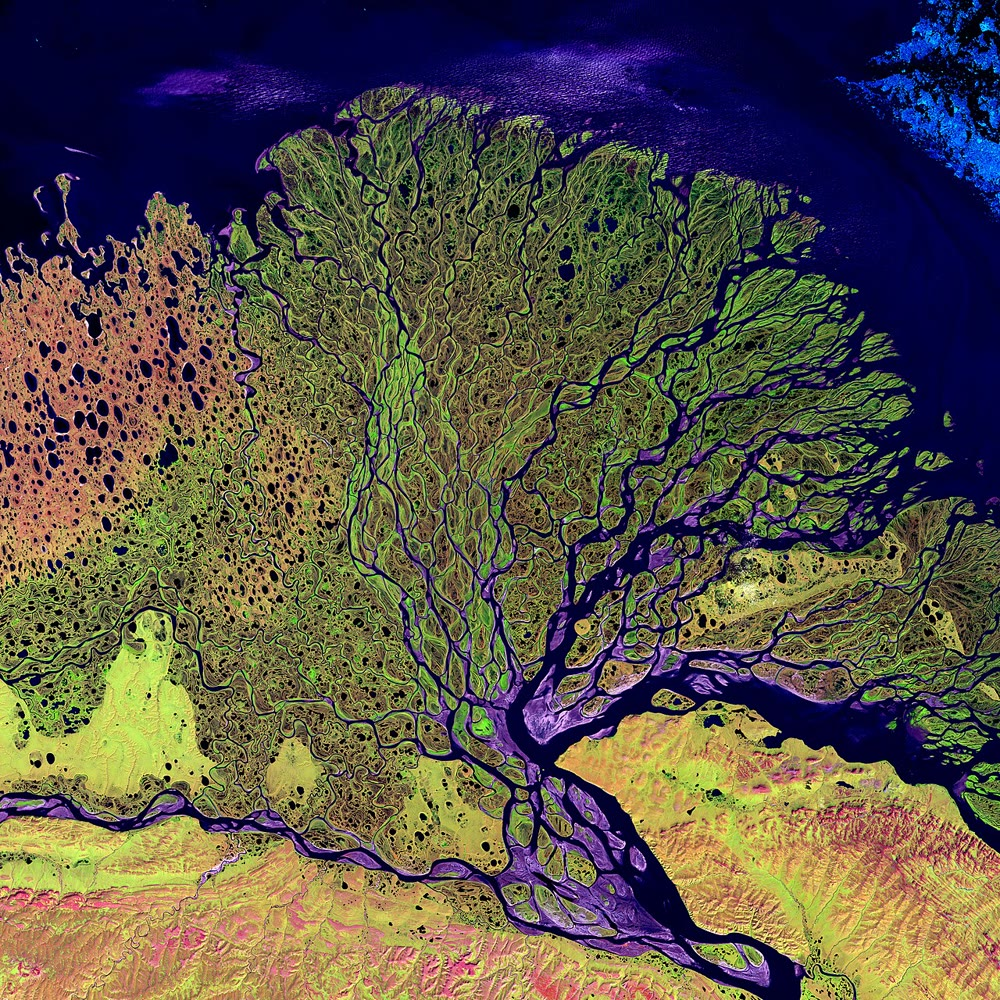
\includegraphics[width=\linewidth]{images/book1/g9-lena-delta.jpg}
\end{minipage}\hfill
\begin{minipage}[c]{0.46\linewidth}\raggedright
{\small Le \omterm{def:g5:water-shapes-the-land:delta}{delta} de la Lena, en Sibérie, là où le fleuve rejoint l'\omterm{def:g2:water-on-earth:ocean}{océan}
Arctique~: une image Landsat en fausses couleurs du 27~février 2000,
réalisée avec l'infrarouge à ondes courtes, l'infrarouge et la lumière
rouge. Les nombreux bras du fleuve apparaissent en bleu. USGS EROS Data
Center, via NASA Visible Earth (domaine public, via Wikimedia Commons).}
\end{minipage}
% ledger: commons:lena-landsat
\label{fig:g9:maps-of-the-earth:lena}
\end{omfigure}

\section{Le positionnement par satellite}

Un téléphone ou une voiture peut savoir où il se trouve à quelques mètres
près, presque partout sur la Terre. Il ne voit pas les satellites~: il les
écoute.

\begin{definition}[Positionnement par satellite]\label{def:g9:maps-of-the-earth:positioning}
Le \emph{positionnement par satellite}\index{positionnement par satellite} consiste à trouver une
position sur la Terre à partir des distances à plusieurs satellites dont
les positions sont connues. Un récepteur calcule chaque distance à partir
du temps que met un signal du satellite pour lui parvenir.
\end{definition}

Le système américain, le GPS, maintient au moins 24 satellites en service
à une \omterm{def:g4:world-physical-map:altitude}{altitude} d'environ \qty{20200}{km}. Chacun fait le tour de la Terre
deux fois par jour, sur six orbites réparties autour de la planète, de
sorte que depuis presque n'importe quel point de la Terre, au moins quatre
satellites sont visibles. Un signal parti de \qty{20200}{km}, voyageant à
la vitesse de la lumière, arrive au bout de $20\,200 \div
300\,000 \approx 0.067$~s~: le récepteur mesure ce temps et le convertit
en distance.
% ledger: gps:constellation, const:c (travel time computed in figdata/grade-9/trilateration.py)

Comment des distances donnent-elles une position~? Représentons-nous
l'idée sur une \omterm{def:g2:drawing-to-map:map}{carte} plane. Si le récepteur est à \qty{5}{km} de la
balise~A, il se trouve quelque part sur un cercle de rayon \qty{5}{km}
autour de A. S'il est aussi à \qty{10}{km} de B, il se trouve sur les deux
cercles~: en l'un des deux points où ils se coupent. Une troisième
distance, \qty{5}{km} de C, désigne le bon. Dans l'espace, les cercles
deviennent des sphères, et il faut un satellite de plus pour la même
raison.

\begin{omfigure}
\begin{minipage}[c]{0.5\linewidth}\centering
\begin{tikzpicture}
\begin{axis}[x=0.42cm, y=0.42cm, xmin=-1, xmax=13, ymin=-1.5, ymax=13,
  ticks=none, axis line style={black!40}]
  \addplot[omSea!70!black, line width=0.6pt] table {figdata/out/grade-9-trilateration-circles.dat};
  \addplot[only marks, mark=triangle*, mark size=2.6pt, point meta=explicit symbolic, nodes near coords,
    nodes near coords style={font=\footnotesize\bfseries, anchor=south west, inner sep=1pt}]
    table[meta=label] {figdata/out/grade-9-trilateration-beacons.dat};
  % labels first (on a white patch), then the points on top of them
  \addplot[only marks, mark=none, point meta=explicit symbolic, nodes near coords,
    nodes near coords style={font=\footnotesize\bfseries, anchor=north east, xshift=-1pt, yshift=-1pt, inner sep=1pt, fill=white, text=red!75!black}, skip coords between index={1}{2}]
    table[meta=label] {figdata/out/grade-9-trilateration-points.dat};
  \addplot[only marks, mark=none, point meta=explicit symbolic, nodes near coords,
    nodes near coords style={font=\footnotesize, anchor=south west, xshift=1pt, yshift=1pt, inner sep=1pt, fill=white}, skip coords between index={0}{1}]
    table[meta=label] {figdata/out/grade-9-trilateration-points.dat};
  \addplot[only marks, mark=*, mark size=2pt, red!75!black, skip coords between index={1}{2}] table {figdata/out/grade-9-trilateration-points.dat};
  \addplot[only marks, mark=o, mark size=2pt, fill=white, skip coords between index={0}{1}] table {figdata/out/grade-9-trilateration-points.dat};
\end{axis}
\end{tikzpicture}
\end{minipage}\hfill
\begin{minipage}[c]{0.46\linewidth}\raggedright
{\small Le positionnement sur une \omterm{def:g2:drawing-to-map:map}{carte} plane (un croquis~; quadrillage en
kilomètres non dessiné). Le récepteur R est à \qty{5}{km} de A, à
\qty{10}{km} de B et à \qty{5}{km} de C. Les cercles autour de A et de B se
coupent en R et en un faux point F~; seul R se trouve aussi sur le cercle
autour de C.}
\end{minipage}
% ledger: (invented region: exercise data, figdata/grade-9/trilateration.py)
\label{fig:g9:maps-of-the-earth:trilateration}
\end{omfigure}

\begin{omfigure}
\begin{minipage}[t]{0.48\linewidth}\centering
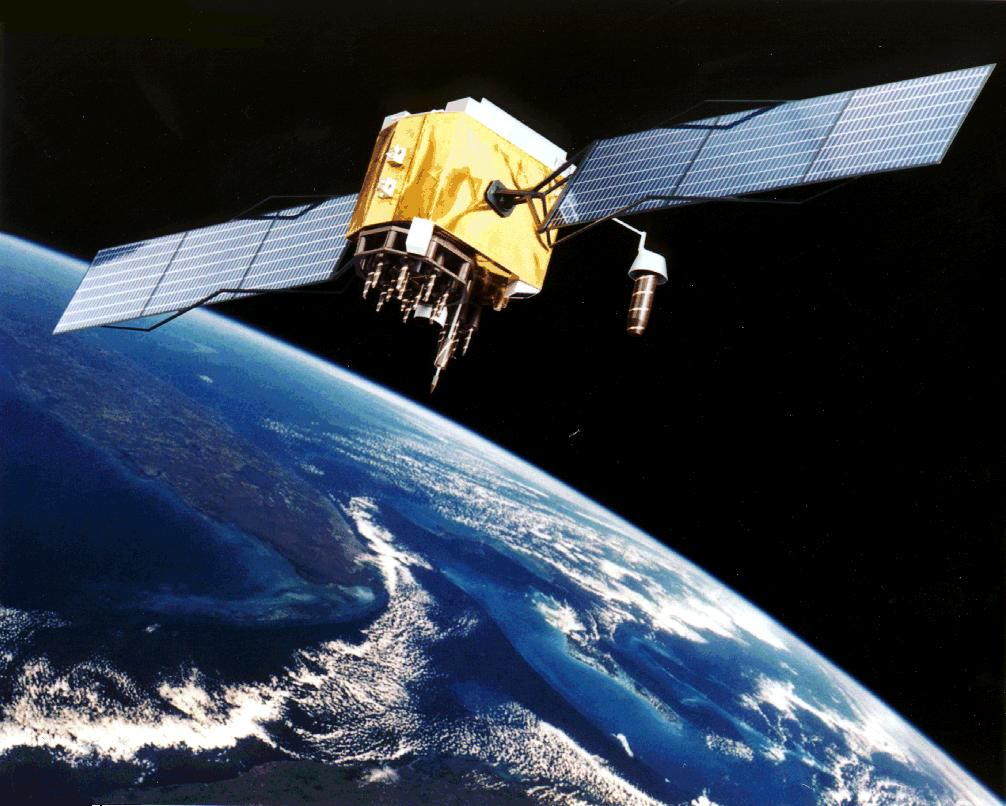
\includegraphics[width=\linewidth]{images/book1/g9-gps-satellite.jpg}

{\small Un satellite GPS en orbite, tel qu'un artiste l'a imaginé. NASA
(domaine public, via Wikimedia Commons).}
\end{minipage}\hfill
\begin{minipage}[t]{0.48\linewidth}\centering
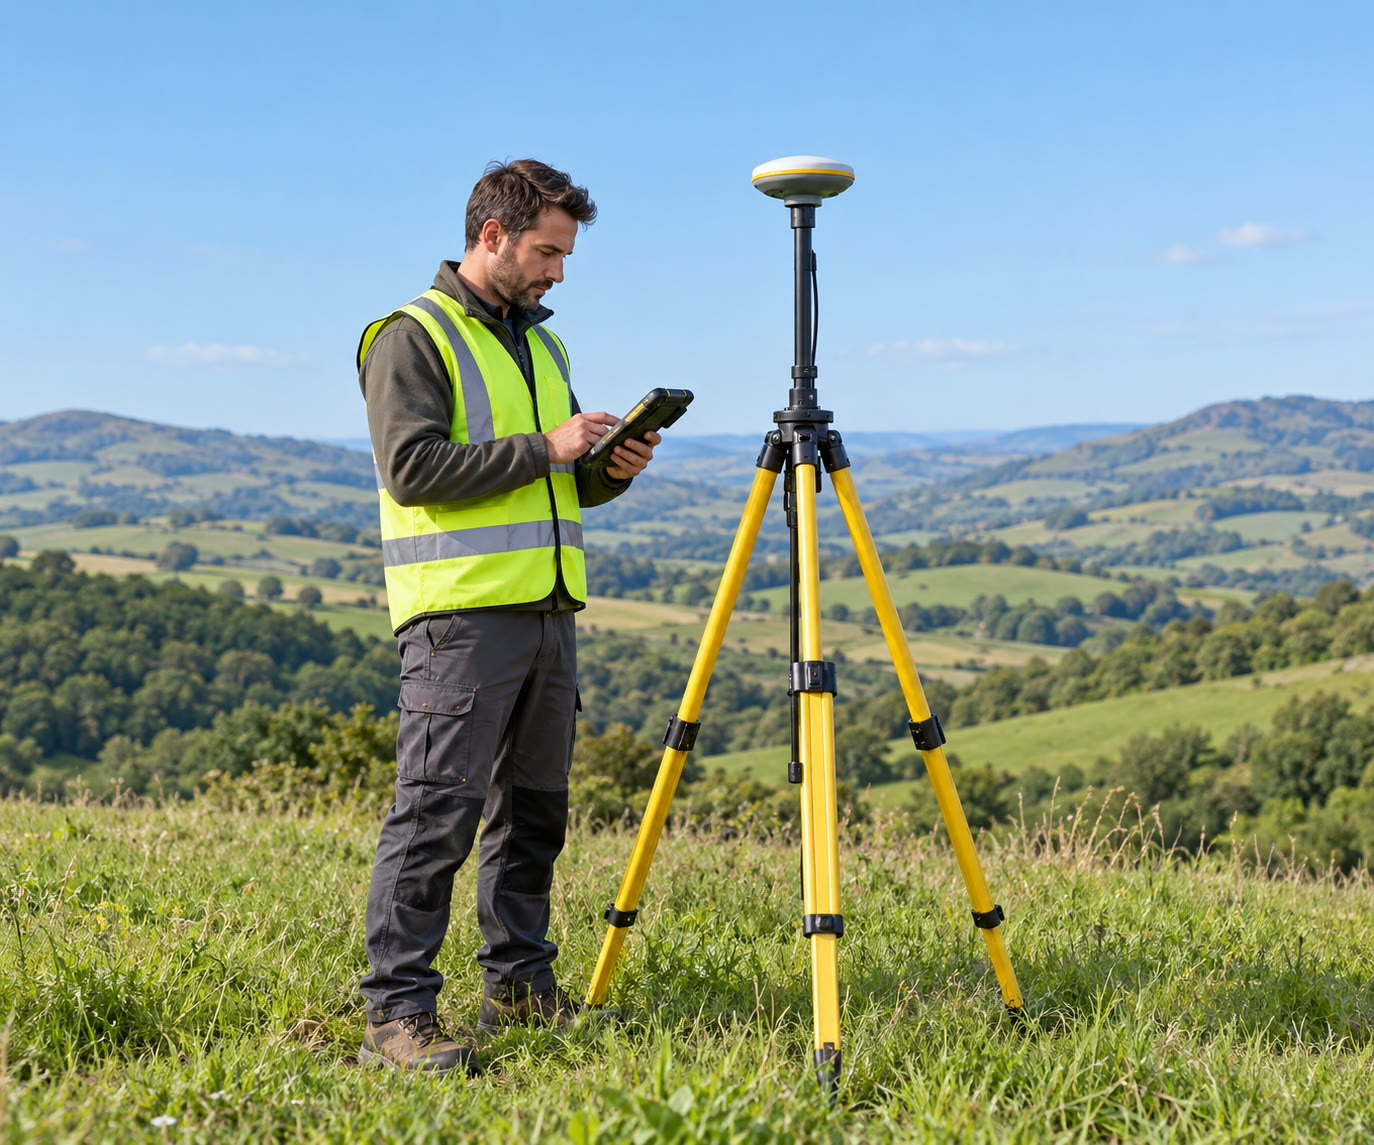
\includegraphics[width=\linewidth]{images/book1/ai/g9-surveyor.jpg}

{\small Un géomètre détermine la position d'un point avec un récepteur
satellite monté sur un trépied (une illustration).}
\end{minipage}
% ledger: commons:gps-iif
\label{fig:g9:maps-of-the-earth:gps}
\end{omfigure}

\section{Exercices}

\begin{exercise}[$\star$]\label{exo:g9:maps-of-the-earth:1}
Donne le mot qui correspond à chaque description. (a) Une règle qui envoie
chaque point du \omterm{def:g3:continents-and-oceans:globe}{globe} en un point d'une \omterm{def:g2:drawing-to-map:map}{carte} plane. (b) Une ligne qui
relie des points situés à la même \omterm{def:g4:world-physical-map:altitude}{altitude}. (c) Un rapport comme
$1 : 50\,000$. (d) La différence d'\omterm{def:g4:world-physical-map:altitude}{altitude} entre deux \omterm{def:g9:maps-of-the-earth:contour}{courbes de niveau}
voisines. (e) L'observation de la Terre à distance, par exemple depuis un
satellite.
\end{exercise}

\begin{exercise}[$\star$]\label{exo:g9:maps-of-the-earth:2}
Convertis chaque distance sur la \omterm{def:g2:drawing-to-map:map}{carte} en distance sur le terrain, en
mètres ou en kilomètres. (a) \qty{4}{cm} sur une \omterm{def:g2:drawing-to-map:map}{carte} au $1 : 25\,000$.
(b) \qty{3}{cm} sur une \omterm{def:g2:drawing-to-map:map}{carte} au $1 : 50\,000$. (c) \qty{2.5}{cm} sur une
\omterm{def:g2:drawing-to-map:map}{carte} au $1 : 1\,000\,000$. (d) Sur une \omterm{def:g2:drawing-to-map:map}{carte} au
$1 : 25\,000$, combien de centimètres représentent \qty{1}{km}~?
\end{exercise}

\begin{exercise}[$\star$]\label{exo:g9:maps-of-the-earth:3}
Vrai ou faux~? Corrige les phrases fausses. (a) Un \omterm{def:g3:continents-and-oceans:world-map}{planisphère} peut
montrer toute la Terre sans rien déformer. (b) Sur une \omterm{def:g2:drawing-to-map:map}{carte} de Mercator,
le Groenland paraît plus grand qu'il n'est. (c) Sur une \omterm{def:g2:drawing-to-map:map}{carte} équivalente,
les formes sont conservées partout. (d) Une \omterm{def:g9:maps-of-the-earth:numerical-scale}{échelle graphique} reste juste
quand une \omterm{def:g2:drawing-to-map:map}{carte} est agrandie à la photocopieuse.
\end{exercise}

\begin{exercise}[$\star$]\label{exo:g9:maps-of-the-earth:4}
Sur une \omterm{def:g9:maps-of-the-earth:topographic-map}{carte topographique}, (a) que signifient des \omterm{def:g9:maps-of-the-earth:contour}{courbes de niveau} très
serrées~? (b) très espacées~? (c) Que montrent des \omterm{def:g9:maps-of-the-earth:contour}{courbes de niveau}
fermées de plus en plus hautes vers l'intérieur~? (d) Pourquoi deux
\omterm{def:g9:maps-of-the-earth:contour}{courbes de niveau} ne peuvent-elles jamais se croiser~?
\end{exercise}

\begin{exercise}[$\star\star$]\label{exo:g9:maps-of-the-earth:5}
% ledger: data:ne-land (factor 1/cos^2, figdata/grade-9/projections.py)
Sur une \omterm{def:g2:drawing-to-map:map}{carte} de Mercator, les surfaces à la \omterm{def:g6:latitude-longitude:latitude}{latitude} \ang{60} sont
agrandies 4 fois, et à la \omterm{def:g6:latitude-longitude:latitude}{latitude} \ang{30} environ 1.33 fois, par rapport
à l'\omterm{def:g3:continents-and-oceans:equator}{équateur}. (a) Un \omterm{def:g1:landscapes-around-us:water}{lac} de \qty{1000}{km^2} situé à \ang{60}\,N est dessiné
sur la \omterm{def:g2:drawing-to-map:map}{carte}. Un \omterm{def:g1:landscapes-around-us:water}{lac} de l'\omterm{def:g3:continents-and-oceans:equator}{équateur} dessiné avec la même taille a quelle
surface réelle~? (b) Deux îles de même surface réelle se trouvent à \ang{30}
et à \ang{60}. Combien de fois la seconde paraît-elle plus grande que la
première~? (c) Pourquoi la \omterm{def:g2:drawing-to-map:map}{carte} de Mercator ne peut-elle jamais montrer
les \omterm{def:g3:continents-and-oceans:poles}{pôles}~?
\end{exercise}

\begin{exercise}[$\star\star$]\label{exo:g9:maps-of-the-earth:6}
% ledger: (invented region: the Varden Hills map of the chapter)
Utilise la \omterm{def:g9:maps-of-the-earth:topographic-map}{carte topographique} des collines de Varden de ce chapitre.
(a) Quelle est l'\omterm{def:g9:maps-of-the-earth:contour}{équidistance}~? (b) Quelle est l'\omterm{def:g4:world-physical-map:altitude}{altitude} du sommet marqué
par son point coté, et celle de la courbe maîtresse qui l'entoure~?
(c) La \omterm{def:g1:landscapes-around-us:water}{rivière} coule vers l'est. Le fond de la \omterm{def:g1:landscapes-around-us:landform}{vallée} est-il plus haut à
l'ouest ou à l'est de la \omterm{def:g2:drawing-to-map:map}{carte}~? (d) Le long de C--D, au nord de la
\omterm{def:g1:landscapes-around-us:water}{rivière}, entre quelles \omterm{def:g9:maps-of-the-earth:contour}{courbes de niveau} les lignes sont-elles le plus
serrées~? Qu'est-ce que cela t'apprend sur la pente à cet endroit~?
\end{exercise}

\begin{exercise}[$\star\star$]\label{exo:g9:maps-of-the-earth:7}
% ledger: (invented region: profile C--D, figdata/grade-9/varden_topo.py)
Utilise le profil C--D de ce chapitre. (a) À peu près à quelle \omterm{def:g4:world-physical-map:altitude}{altitude} se
trouvent C et D~? (b) Quelle est l'\omterm{def:g4:world-physical-map:altitude}{altitude} la plus basse le long du
profil, et à quelle distance de C se trouve-t-elle~? (c) Quelle est la
longueur du fond de \omterm{def:g1:landscapes-around-us:landform}{vallée} plat le long de C--D~? (d) Le profil est tracé
avec une échelle verticale exagérée trois fois. Pourquoi les cartographes
le font-ils souvent~?
\end{exercise}

\begin{exercise}[$\star\star$]\label{exo:g9:maps-of-the-earth:8}
Sur une \omterm{def:g2:drawing-to-map:map}{carte} au $1 : 25\,000$, un sentier coupe la courbe de \qty{200}{m}
puis celle de \qty{300}{m}, \qty{2}{cm} plus loin. (a) Quelle est la
distance horizontale entre les deux points sur le terrain~? (b) De
combien le sentier monte-t-il~? (c) Quelle est la pente, en
pourcentage~? (d) Plus loin, deux courbes distantes de \qty{100}{m} en
\omterm{def:g4:world-physical-map:altitude}{altitude} sont séparées de \qty{4}{cm} sur la \omterm{def:g2:drawing-to-map:map}{carte}. Le sentier y est-il
plus raide ou moins raide~? De combien~?
\end{exercise}

\begin{exercise}[$\star\star$]\label{exo:g9:maps-of-the-earth:9}
% ledger: usgs:landsat1
Landsat~1 faisait le tour de la Terre 14 fois par jour et repassait
au-dessus du même lieu tous les 18 jours. (a) Combien d'orbites
faisait-il entre deux passages au-dessus du même lieu~? (b) Chaque orbite
durait 103 minutes. Combien d'heures durent 14 orbites~? (c) Conçu pour
fonctionner un an, il fut éteint le 6~janvier 1978, cinq ans et demi
après son lancement. Combien de fois sa durée de vie prévue a-t-il
fonctionné~? (d) Donne un changement de la surface de la Terre que
peuvent montrer des images d'un même lieu prises à des années
d'intervalle.
\end{exercise}

\begin{exercise}[$\star\star$]\label{exo:g9:maps-of-the-earth:10}
% ledger: gps:constellation, const:c
Un satellite GPS se trouve à environ \qty{20200}{km}~; son signal se
propage à environ \qty{300000}{km} par seconde. (a) Combien de temps le
signal met-il à arriver~? Écris la réponse en notation scientifique.
(b) Si l'horloge d'un récepteur se trompait de $1 \times 10^{-3}$~s,
quelle erreur sur la distance cela produirait-il~? (c) Qu'est-ce que cela
t'apprend sur les horloges utilisées pour le \omterm{def:g9:maps-of-the-earth:positioning}{positionnement par
satellite}~?
\end{exercise}

\begin{exercise}[$\star\star\star$]\label{exo:g9:maps-of-the-earth:11}
Sur une \omterm{def:g2:drawing-to-map:map}{carte} plane quadrillée en kilomètres, la balise A est en $(0, 0)$
et la balise B en $(10, 0)$. Un récepteur est à \qty{6}{km} de A et à
\qty{8}{km} de B. (a) Montre que le point $(3.6, 4.8)$ est à \qty{6}{km} de A
et à \qty{8}{km} de B. (b) Donne un autre point situé aux mêmes distances
de A et de B. (c) Une troisième balise C est en $(0, 10)$, et le récepteur
en est à environ \qty{6.3}{km}. Lequel des deux points est le récepteur~?
(d) Pourquoi le \omterm{def:g9:maps-of-the-earth:positioning}{positionnement par satellite} a-t-il besoin de plusieurs
satellites~?
\end{exercise}

\begin{exercise}[$\star\star\star$]\label{exo:g9:maps-of-the-earth:12}
% ledger: data:ne-land (areas, figdata/grade-9/projections.py)
L'Afrique continentale couvre environ 29~millions de~\unit{km^2} et le
Groenland environ 2.1~millions de~\unit{km^2}. (a) Combien de fois
l'Afrique est-elle plus grande~? (b) Sur une \omterm{def:g2:drawing-to-map:map}{carte} de Mercator, les
surfaces proches du milieu du Groenland, à environ \ang{72}\,N, sont
agrandies environ 10.5 fois. Estime la surface que le Groenland semble
avoir. (c) L'Afrique s'étend de part et d'autre de l'\omterm{def:g3:continents-and-oceans:equator}{équateur}, où les
surfaces sont peu agrandies. Compare ta réponse à (b) avec la surface de
l'Afrique, et explique la \omterm{def:g2:drawing-to-map:map}{carte} murale du début du chapitre. (d) Quelle
projection choisirais-tu pour montrer équitablement la taille des
\omterm{def:g3:continents-and-oceans:continent}{continents}~?
\end{exercise}

\section{Problème~: un sentier à travers les collines de Varden}

\begin{problem}[{Problème du week-end --- des aménageurs ont tracé un
sentier à travers les collines de Varden sur la carte topographique~; la
réponse finale est la longueur du sentier en kilomètres et sa dénivelée
positive totale en mètres}]
\label{pb:g9:maps-of-the-earth:1}
% ledger: (invented region: the Varden Hills, figdata/grade-9/varden_topo.py, part problem: leg lengths 3.6 / 2.5 / 2.35 cm, spot heights 296 / 143 / 335 / 544 m, 4.2 km, 401 m)
Le sentier part d'une ferme S, descend jusqu'à un pont B sur la \omterm{def:g1:landscapes-around-us:water}{rivière},
puis monte jusqu'à un abri W et continue jusqu'au sommet T. Chaque tronçon
est rectiligne et ne fait que descendre ou que monter. La \omterm{def:g2:drawing-to-map:map}{carte} est au
$1 : 50\,000$~; les \omterm{def:g4:world-physical-map:altitude}{altitudes} de S, B, W et T sont écrites à côté d'eux.

\begin{omfigure}
\begin{tikzpicture}
\begin{axis}[x=1.6cm, y=1.6cm, xmin=2, xmax=8, ymin=1.8, ymax=6.2, ticks=none,
  axis line style={black!60}, clip mode=individual]
  \addplot[contour] table {figdata/out/shared-region-contours.dat};
  \addplot[index contour] table {figdata/out/shared-region-index-contours.dat};
  \addplot[river] table {figdata/out/shared-region-river.dat};
  \addplot[only marks, mark=none, point meta=explicit symbolic, nodes near coords,
    nodes near coords align={center}, nodes near coords style={font=\tiny, fill=white, inner sep=0.6pt, text=omContour}]
    table[meta=label] {figdata/out/grade-9-varden_topo-labels.dat};
  \addplot[red!75!black, line width=1pt, dashed] table[x=x_km, y=y_km] {figdata/out/grade-9-varden_topo-path.dat};
  \addplot[only marks, mark=*, mark size=1.6pt, red!75!black, point meta=explicit symbolic, nodes near coords,
    nodes near coords align={right}, nodes near coords style={font=\scriptsize\bfseries, text=black, fill=white, fill opacity=0.8, text opacity=1, inner sep=1pt}]
    table[meta=label] {figdata/out/grade-9-varden_topo-points.dat};
  \coordinate (na) at (axis cs:8.35,5.4);
\end{axis}
\pic at (na) {northarrow};
\end{tikzpicture}

{\small Le sentier S--B--W--T sur la \omterm{def:g9:maps-of-the-earth:topographic-map}{carte topographique} des collines de
Varden (représentée ici en réduction~; sur la \omterm{def:g2:drawing-to-map:map}{carte} originale au
$1 : 50\,000$, les tronçons mesurent 3.6, 2.5 et \qty{2.35}{cm}).}
\label{fig:g9:maps-of-the-earth:path}
\end{omfigure}

\noindent\textbf{Partie I --- L'itinéraire sur la carte.}\par\nopagebreak
\begin{enumerate}[beginpenalty=10000]
  \item Au $1 : 50\,000$, combien de mètres sur le terrain représente
        \qty{1}{cm} de la \omterm{def:g2:drawing-to-map:map}{carte}~?
  \item Sur la \omterm{def:g2:drawing-to-map:map}{carte} originale, le tronçon S--B mesure \qty{3.6}{cm}.
        Quelle est sa longueur sur le terrain, en kilomètres~?
  \item Les tronçons B--W et W--T mesurent \qty{2.5}{cm} et
        \qty{2.35}{cm}. Quelle est leur longueur sur le terrain~?
  \item Dans quelle direction générale le sentier va-t-il de B à T~?
\end{enumerate}

\noindent\textbf{Partie II --- La montée.}\par\nopagebreak
\begin{enumerate}[resume, beginpenalty=10000]
  \item Quelle est l'\omterm{def:g9:maps-of-the-earth:contour}{équidistance} de la \omterm{def:g2:drawing-to-map:map}{carte}~?
  \item Quel tronçon descend~? De combien de mètres~?
  \item De combien de mètres le sentier monte-t-il sur B--W, et sur W--T~?
  \item Quelle est la pente moyenne du tronçon W--T, en pourcentage~?
  \item Pourquoi les aménageurs n'ont-ils pas tracé le sentier en ligne
        droite de S à T~?
\end{enumerate}

\noindent\textbf{Partie III --- La marche.}\par\nopagebreak
\begin{enumerate}[resume, beginpenalty=10000]
  \item Suppose qu'un randonneur parcoure \qty{4}{km} par heure sur le plat
        et ait besoin d'une minute de plus pour chaque \qty{10}{m} de
        montée. Combien de temps dure toute la marche~?
  \item Une autre randonneuse suit le sentier dans l'autre sens, de T à S.
        De combien de mètres monte-t-elle~?
  \item Quelle est la longueur totale du sentier, en kilomètres, et sa
        dénivelée positive totale, en mètres~?
\end{enumerate}
\end{problem}
